\subsection{Template Method}

\subsubsection*{Problembeschreibung}

Es existieren ein Algorithmus, welcher aus einer Menge von Teilschritten besteht. Die einzelnen Teilschritte sollen austauschbar gehalten werden, um ein flexibles Anpassen des Algorithmus zu ermöglichen. Die Reihenfolge der Teilschritte ist hingegen festgelegt. 

\subsubsection*{Lösung}

\begin{figure}[!hb]
	\centering
	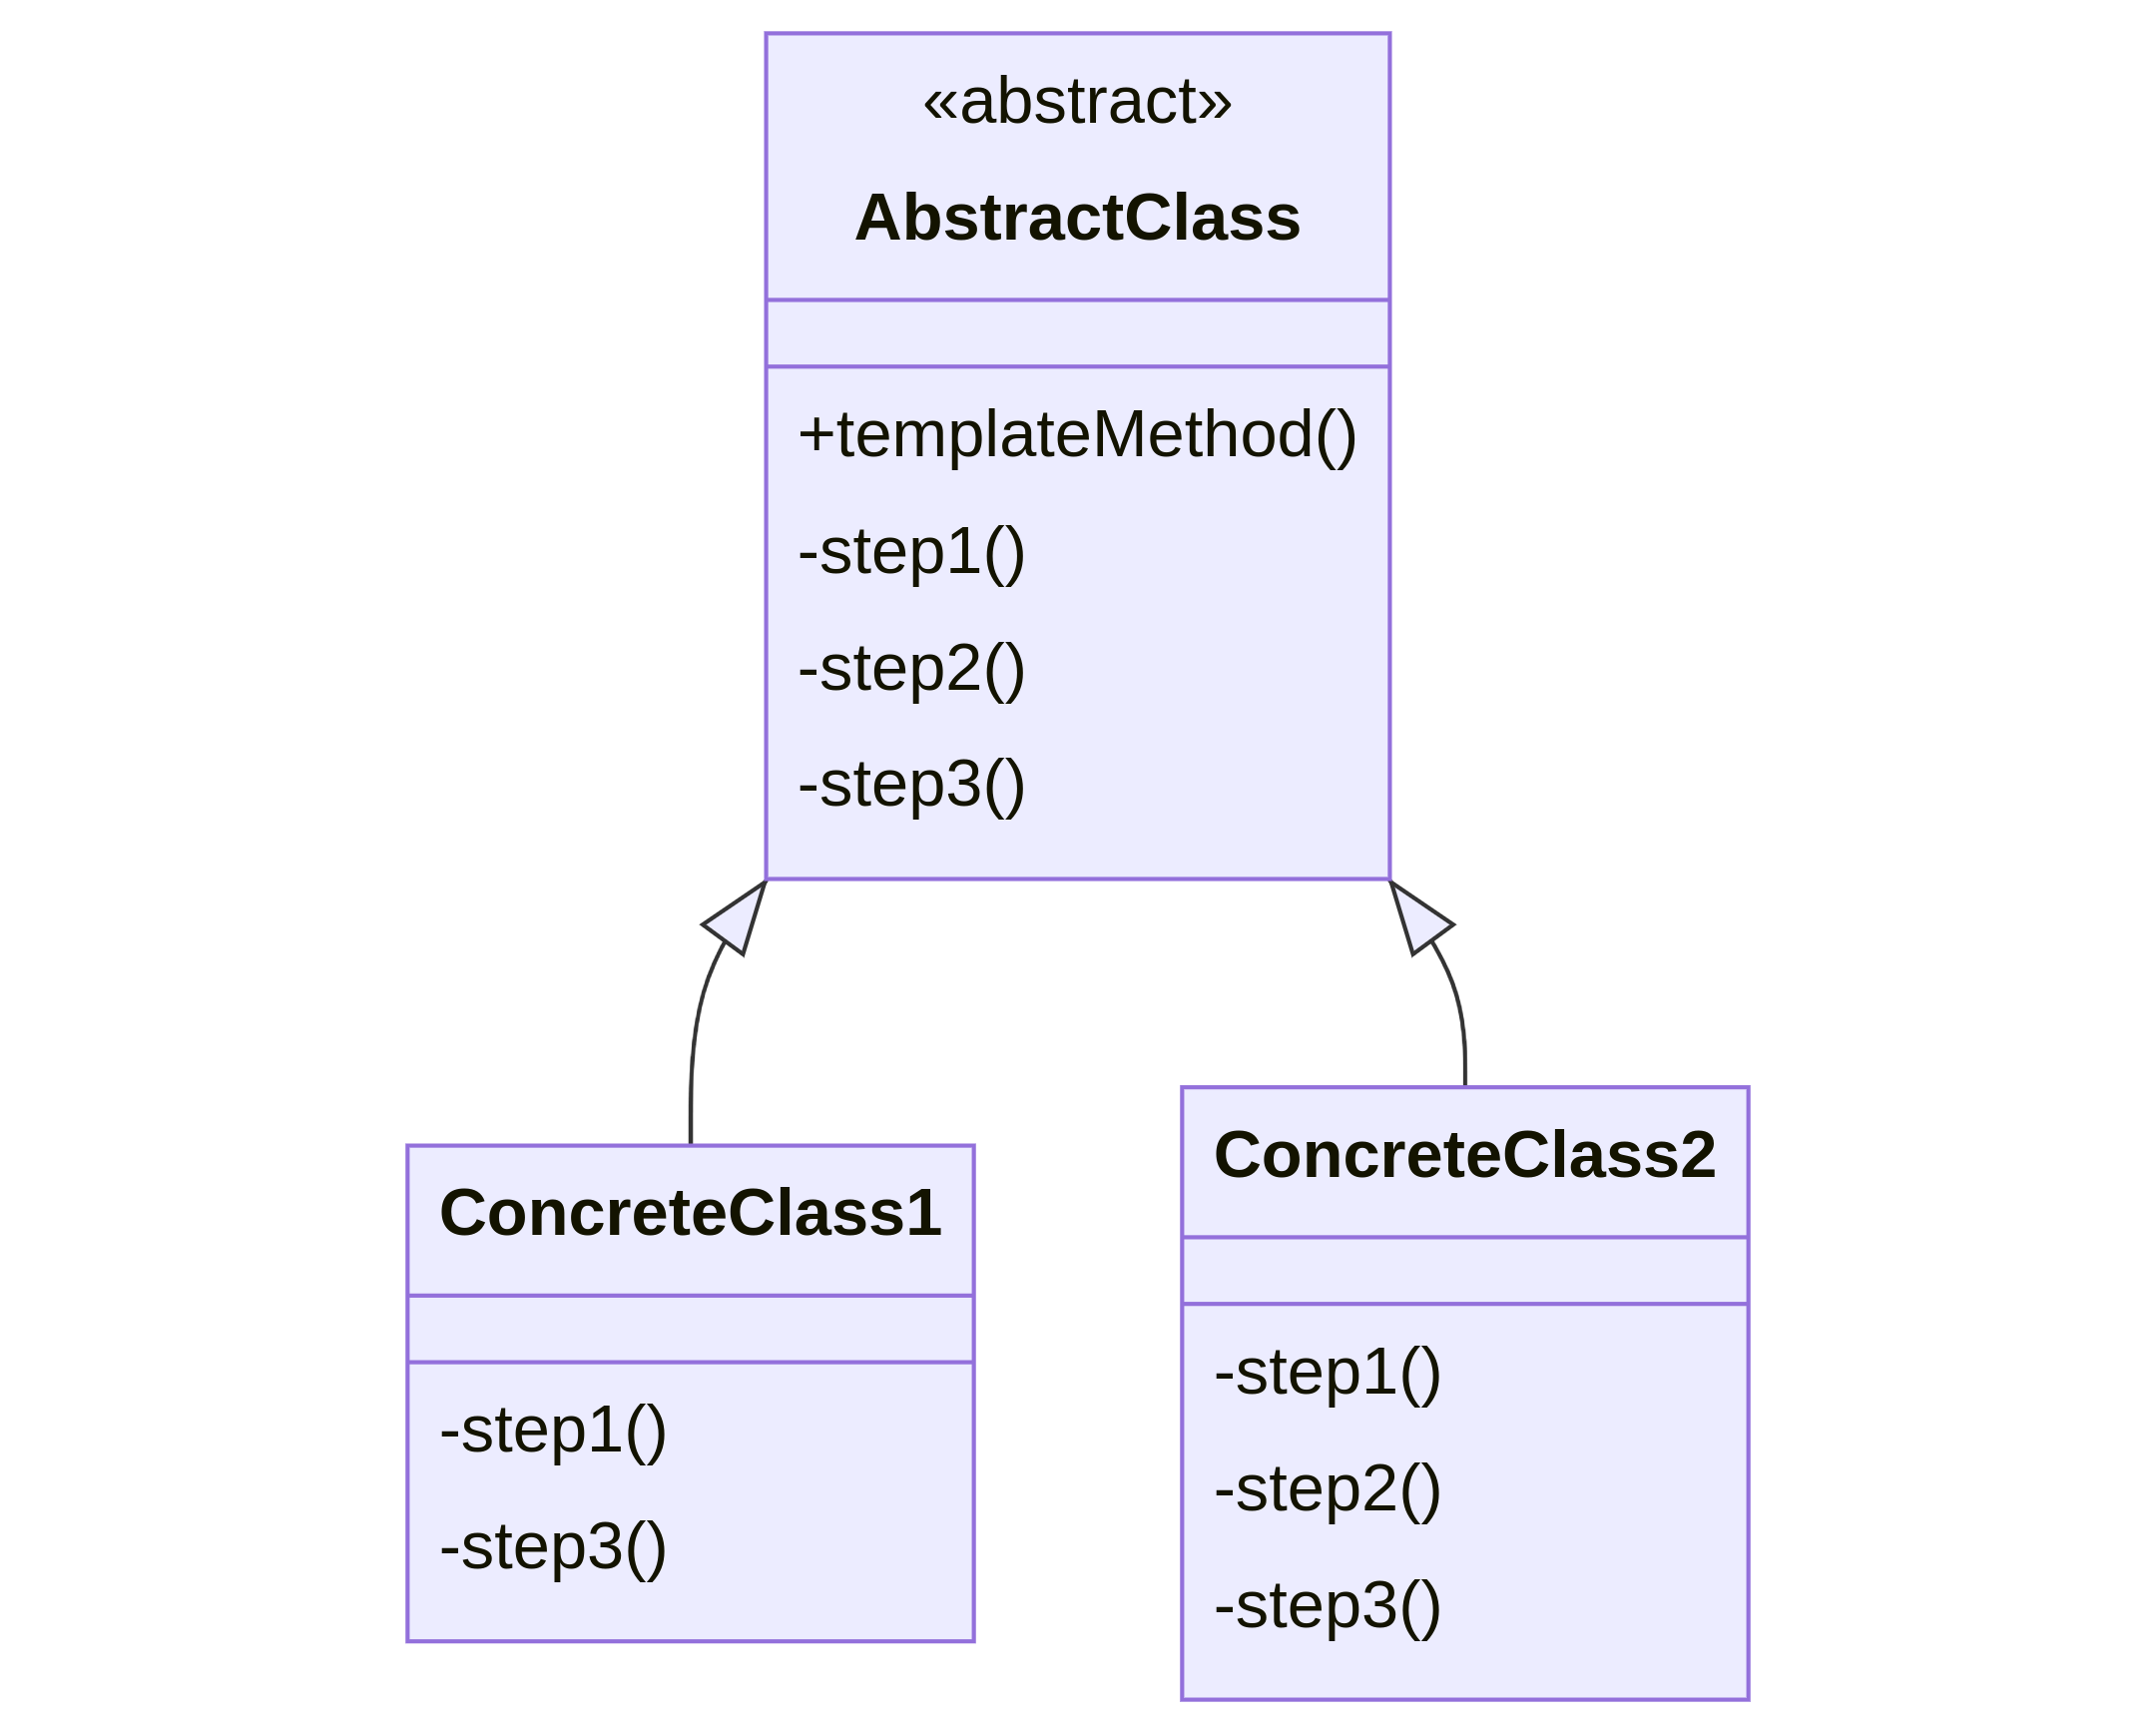
\includegraphics[width=0.75\linewidth]{images/patterns/template-method-class.png}
	\caption{Klassendiagramm Template Method}
	\label{fig:template-method-class}
\end{figure}

Jede Klasse, welche einen Algorithmus der selben Struktur implementiert, erbt von einer abstrakten Klassen, welche die `templateMethod` implementiert. Diese gibt das Grundgerüst des Algorithmus vor und ruft darin die einzelnen Teilschritte auf. Diese sind jeweils in eigenen Methoden implementiert. Die Subklassen definieren diese Methoden zum Teil neu, wenn eine Veränderung des Verhaltens dieses Teilschrittes notwendig ist.


\lstset{language=python}
\begin{lstlisting}[caption={Quelltextunterschrift}, label=code:template-method-code]
class AbstractClass:
	def templateMethod(self):
    	if self.step1():
        	self.step2()
    	self.step3()
\end{lstlisting}


\subsubsection*{Konsequenzen}

Template Methods sind ein Mechanismus, welcher die Wiederverwendung von Code ermöglicht und kann somit der Codeduplikation entgegen wirken. Anstatt Abwandlungen von Algorithmen von Grund auf neu zu implementieren, ist es möglich, sie aus bestehenden Komponenten zusammenzusetzen und je nach Bedarf neuen Code hinzuzufügen. Das Muster der Template-Method weist eine umgekehrte Kontrollstruktur auf. Anstatt dass eine Klasse Methoden ihrer Superklasse aufruft, delegiert die Template-Method die Verantwortlichkeit für die einzelnen Teile des Algorithmus an sie Subklassen.

Bei der Verwendung der Template-Method ist jedoch zu beachten, wie die einzelnen Methoden zu verwenden sind. Diese lassen sich grob in zwei Arten einteilen, Die "Hook"-Methoden und die abstrakten Methoden. Während die "Hook"-Methoden eine Standard-Implementierung in der abstrakten Basisklasse bereitstellen, ist dies bei den abstrakten Methoden nicht der Fall. Entsprechend müssen die abstrakten Methoden zwingend von einer konkreten Subklasse implementiert werden. Bei den "Hook"-Methoden ist das optional. 

Die Template-Method synergiert mit dem Strategy-Pattern. Einzelne Schritte eine Algorithmus können in einer Strategie-Klasse implementiert sein.